\documentclass[wide,a4paper,titlepage,12pt] {article}
\usepackage{polski}
\usepackage[utf8]{inputenc}
\usepackage{listings}
\usepackage{slashbox}
\usepackage[table]{xcolor}
\usepackage{graphicx,pdflscape}
\usepackage{placeins}


\title{Urządzenia peryferyjne}
\author{Tymon Tobolski (181037)\\ Jacek Wieczorek (181043)}

% Title page layout (fold)
\makeatletter
\renewcommand{\maketitle}{
\begin{titlepage}
  \begin{center}
    \vspace*{3cm}
    \LARGE \@title \par
    \vspace{2cm}
    \textit{\small Autor:}\par
    \normalsize \@author\par \normalsize
    \vspace{3cm}
    \textit{\small Prowadzący:}\par
    Dr inż. Jacek Mazurkiewicz \par
    \vspace{2cm}
    Wydział Elektroniki\\ III rok\\ Pn 8.15 - 11.00\par
    \vspace{4cm}
    \small \@date
  \end{center}
\end{titlepage}
}
\makeatother



\begin{document}
\maketitle

\section{Cel laboratorium}
\paragraph{}
Celem laboratorium było zapoznanie się z zasdą pracy i obsługą skanera płaskiego.

\section{Program}


% \lstset{ %
%     language=java,                % choose the language of the code
%     basicstyle=\scriptsize,       % the size of the fonts that are used for the code
%     numbers=left,                   % where to put the line-numbers
%     numberstyle=\scriptsize,      % the size of the fonts that are used for the line-numbers
%     stepnumber=10,                   % the step between two line-numbers. If it's 1 each line 
%                                     % will be numbered
%     numbersep=9pt,                  % how far the line-numbers are from the code
%     % backgroundcolor=\color{white},  % choose the background color. You must add \usepackage{color}
%     showspaces=false,               % show spaces adding particular underscores
%     showstringspaces=false,         % underline spaces within strings
%     showtabs=false,                 % show tabs within strings adding particular underscores
%     % frame=single,                 % adds a frame around the code
%     % tabsize=2,                  % sets default tabsize to 2 spaces
%     % captionpos=b,                   % sets the caption-position to bottom
%     breaklines=true,                % sets automatic line breaking
%     % breakatwhitespace=false,        % sets if automatic breaks should only happen at whitespace
%     % title=\lstname,                 % show the filename of files included with \lstinputlisting;
%                                     % also try caption instead of title
%     % escapeinside={\%*}{*)},         % if you want to add a comment within your code
%     % morekeywords={*,...}            % if you want to add more keywords to the set
%     }
%     \lstinputlisting{p1.cs}


% \subsection{GUI aplikacji}
% \begin{figure}[htbp]
%       \begin{center}
%        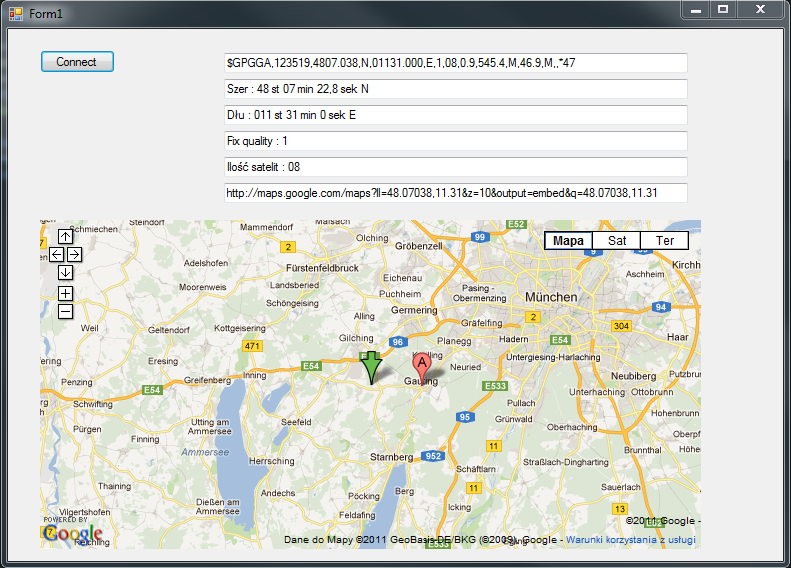
\includegraphics[width=\textwidth]{screen.PNG}
% 	\label{fig5}
% 	\caption{Przykładowe okno programu}
%       \end{center}
%     \end{figure}
\section{Wnioski}
\paragraph{}
\end{document}